% Figure: one account record, held in the SAM hive or in NTDS.dit.
% Used in section 2.1. Values are illustrative, not taken from a real host.
% Two complete cards, not two columns of one table: each store shows only the
% fields it keeps. The grey band crosses both cards and the gap because the
% rows it covers are the fields both stores hold, at the same height.
\begin{figure}[H]
\centering
\footnotesize
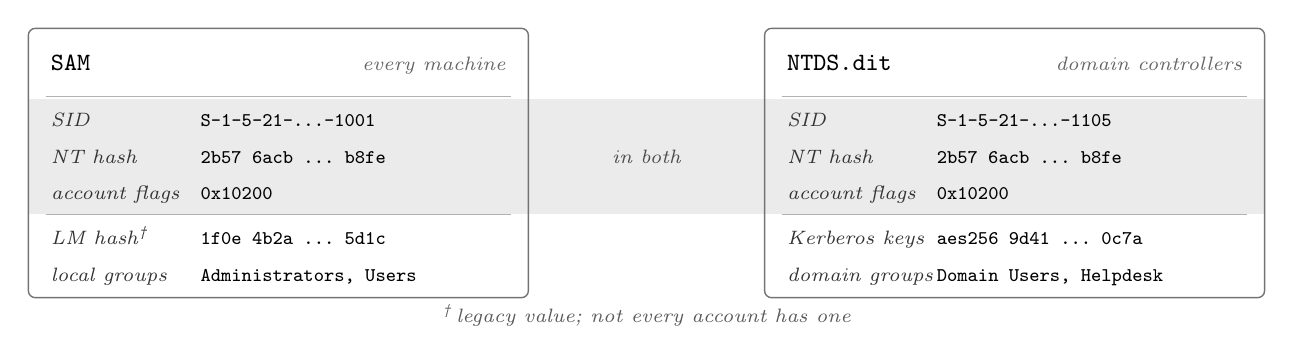
\begin{tikzpicture}[x=1cm,y=1cm,
  card/.style={draw=black!55, line width=0.5pt, rounded corners=2.5pt},
  head/.style={font=\small\ttfamily\bfseries, anchor=base west, inner sep=0pt},
  scope/.style={font=\scriptsize\itshape, text=black!60, anchor=base east,
                inner sep=0pt},
  field/.style={font=\scriptsize\itshape, text=black!80, anchor=base west,
                inner sep=0pt},
  val/.style={font=\scriptsize\ttfamily, anchor=base west, inner sep=0pt}
]

% the shared fields: one band, drawn first so it runs behind both cards
\fill[black!8] (0,-0.90) rectangle (15.7,-2.36);

% the two cards
\draw[card] (0,0) rectangle (6.35,-3.42);
\draw[card] (9.35,0) rectangle (15.7,-3.42);

% header rules and the rule that closes the shared block
\draw[black!30, line width=0.4pt] (0.22,-0.86) -- (6.13,-0.86);
\draw[black!30, line width=0.4pt] (9.57,-0.86) -- (15.48,-0.86);
\draw[black!30, line width=0.4pt] (0.22,-2.36) -- (6.13,-2.36);
\draw[black!30, line width=0.4pt] (9.57,-2.36) -- (15.48,-2.36);

% card headings: store, and the scope it covers
\node[head]  at (0.28,-0.53) {SAM};
\node[scope] at (6.07,-0.53) {every machine};
\node[head]  at (9.63,-0.53) {NTDS.dit};
\node[scope] at (15.42,-0.53) {domain controllers};

% the band's label sits in the gap, on the band itself
\node[font=\scriptsize\itshape, text=black!70, anchor=base]
  at (7.85,-1.71) {in both};

% ---- left card: local account, SAM hive ------------------------------
\node[field] at (0.28,-1.25) {SID};
\node[val]   at (2.18,-1.25) {S-1-5-21-\dots-1001};
\node[field] at (0.28,-1.71) {NT hash};
\node[val]   at (2.18,-1.71) {2b57 6acb \dots\ b8fe};
\node[field] at (0.28,-2.17) {account flags};
\node[val]   at (2.18,-2.17) {0x10200};

\node[field] at (0.28,-2.75) {LM hash\smash{\textsuperscript{\dag}}};
\node[val]   at (2.18,-2.75) {1f0e 4b2a \dots\ 5d1c};
\node[field] at (0.28,-3.21) {local groups};
\node[val]   at (2.18,-3.21) {Administrators, Users};

% ---- right card: domain account, NTDS.dit ----------------------------
\node[field] at (9.63,-1.25) {SID};
\node[val]   at (11.53,-1.25) {S-1-5-21-\dots-1105};
\node[field] at (9.63,-1.71) {NT hash};
\node[val]   at (11.53,-1.71) {2b57 6acb \dots\ b8fe};
\node[field] at (9.63,-2.17) {account flags};
\node[val]   at (11.53,-2.17) {0x10200};

\node[field] at (9.63,-2.75) {Kerberos keys};
\node[val]   at (11.53,-2.75) {aes256 9d41 \dots\ 0c7a};
\node[field] at (9.63,-3.21) {domain groups};
\node[val]   at (11.53,-3.21) {Domain Users, Helpdesk};

% honesty about the legacy value, without cluttering either card
\node[font=\scriptsize\itshape, text=black!65, anchor=base]
  at (7.85,-3.74)
  {\textsuperscript{\dag}\,legacy value; not every account has one};

\end{tikzpicture}
\caption{One account record, two homes.}
\label{fig:two-stores}
\end{figure}
